%%%%%%%%%%%%%%%%%%%%%%%%%%%%%% -*- Mode: Latex -*- %%%%%%%%%%%%%%%%%%%%%%%%%%%%
%% 04-14-appendix.tex -- 
%% Author          : Aaron A. Kagawa
%% Created On      : Tue Sept 21 12:04:50 2004
%% Last Modified By: Aaron Kagawa
%% Last Modified On: Tue Dec  7 23:01:04 2004
%% Status          : Unknown
%% RCS: $Id: 04-appendix.tex,v 1.3 2000/03/17 21:28:36 rbrewer Exp $
%%%%%%%%%%%%%%%%%%%%%%%%%%%%%%%%%%%%%%%%%%%%%%%%%%%%%%%%%%%%%%%%%%%%%%%%%%%%%%%
%%   Copyright (C) 1998 Robert Brewer
%%%%%%%%%%%%%%%%%%%%%%%%%%%%%%%%%%%%%%%%%%%%%%%%%%%%%%%%%%%%%%%%%%%%%%%%%%%%%%%
%% 

\appendix

\chapter{Consent Form}
\label{appendix:consent}
\begin{figure}[htbp]
  \centering
  \includegraphics[width=1.0\textwidth]{figs/ConsentForm_shrunk.eps}
  \caption{Consent Form}
  \label{fig:consent}
\end{figure}

\chapter{Questionnaires}
\label{appendix:questionnaire}

\begin{figure}[htbp]
  \centering
  \includegraphics[width=1.0\textwidth]{figs/hackyTelemetry-questionnaire-shrunk_1.eps}
  \caption{Questionnaire - Part 1}
  \label{fig:questionnaire1}
\end{figure}

\begin{figure}[htbp]
  \centering
  \includegraphics[width=0.63\textwidth]{figs/2004-11-18-hackyTelemetry.eps}
  \caption{Questionnaire - Part 2.1}
  \label{fig:questionnaire2.1}
\end{figure}

\begin{figure}[htbp]
  \centering
  \includegraphics[width=1.0\textwidth]{figs/hackyTelemetry-questionnaire-shrunk_2.eps}
  \caption{Questionnaire - Part 2.2}
  \label{fig:questionnaire2.2}
\end{figure}


\chapter{Inpsection Log and Results}
\label{appendix:log}
This appendix provides a journal of my processes throughout the evaluation
of Priority Ranked Inspection (PRI). I include several details about each
inspection that is conducted, which include: the PRI determination, some of 
the measures that PRI used to create the determination, my subjective
opinions about the package to be inspected, the results in terms of the
number of issues found and their severity, and my subjective opinions on
the PRI determination given the results.

Using this journal, I hope to construct a general guidelines for the use of
and calibration of PRI for other organizations and projects.

%\begin{figure}[htbp]
%  \centerline{\psfig{figure=figs/Acceptance.ps}}
%  \caption{Acceptance}
%  \label{fig:acceptance}
%\end{figure}

\begin{figure}[htbp]
  \centering
  \includegraphics[width=1.0\textwidth]{figs/engineeringlog_word_html_1.eps}
  \caption{Inspection Log and Results - Part 1}
  \label{fig:log1}
\end{figure}

\begin{figure}[htbp]
  \centering
  \includegraphics[width=1.0\textwidth]{figs/engineeringlog_word_html_2.eps}
  \caption{Inspection Log and Results - Part 2}
  \label{fig:log2}
\end{figure}

\begin{figure}[htbp]
  \centering
  \includegraphics[width=1.0\textwidth]{figs/engineeringlog_word_html_3.eps}
  \caption{Inspection Log and Results - Part 3}
  \label{fig:log3}
\end{figure}

\begin{figure}[htbp]
  \centering
  \includegraphics[width=1.0\textwidth]{figs/engineeringlog_word_html_4.eps}
  \caption{Inspection Log and Results - Part 4}
  \label{fig:log4}
\end{figure}

\begin{figure}[htbp]
  \centering
  \includegraphics[width=1.0\textwidth]{figs/engineeringlog_word_html_5.eps}
  \caption{Inspection Log and Results - Part 5}
  \label{fig:log5}
\end{figure}

\begin{figure}[htbp]
  \centering
  \includegraphics[width=1.0\textwidth]{figs/engineeringlog_word_html_6.eps}
  \caption{Inspection Log and Results - Part 6}
  \label{fig:log6}
\end{figure}

\begin{figure}[htbp]
  \centering
  \includegraphics[width=1.0\textwidth]{figs/engineeringlog_word_html_7.eps}
  \caption{Inspection Log and Results - Part 7}
  \label{fig:log7}
\end{figure}

\begin{figure}[htbp]
  \centering
  \includegraphics[width=1.0\textwidth]{figs/engineeringlog_word_html_8.eps}
  \caption{Inspection Log and Results - Part 8}
  \label{fig:log8}
\end{figure}

\begin{figure}[htbp]
  \centering
  \includegraphics[width=1.0\textwidth]{figs/engineeringlog_word_html_9.eps}
  \caption{Inspection Log and Results - Part 9}
  \label{fig:log9}
\end{figure}





